\documentclass[14pt, a4paper, titlepage, fleqn]{extarticle}

\usepackage[russian]{babel}

\usepackage{amsmath}
\usepackage{amssymb}
\usepackage{graphicx}
\usepackage{float}
\usepackage{hyperref}

\delimitershortfall=-1pt

\newcommand{\rnc}[1]
    {\MakeUppercase{\romannumeral #1}}

\DeclareMathOperator{\Ei}{Ei}
\DeclareMathOperator{\li}{li}

\title{Лабораторная работа №2 по дисциплине <<Дифференциальные уравнения>>}
\author{Держапольский Юрий Витальевич}
% \date{}

\begin{document}

    \maketitle

    \tableofcontents

    \pagebreak

    \section{Введение}
        В этой лабораторной работе мы будем решать дифференциальные
        уравнения, строить векторные поля, а также решать и проверять задачи Коши,
        верстая решения в \LaTeX.

    \pagebreak

    \section{Задание 1: Решить уравнения}
        \subsection{Постановка задачи}
            Для следующих дифференциальных уравнений определить тип, найти общее
            решение и построить векторное поле с помощью программ компьютерной математики:
            \begin{enumerate}
                \item 
                \( 
                    u' \cdot \ln{x} + 2xu = 2x \cdot \sqrt{u}
                \)
                
                \item 
                \( 
                    e^{xy} \cdot \left( y^2 + xyy' \right) = y' + y \cdot \cot{x}
                \)
                
                \item 
                \( 
                    r' \cdot \cos^2{\varphi} = \sec{r} \cdot \ln{\sin{r}} 
                \)
                
                \item 
                \( 
                    5x\sqrt{x} \cdot u' -5u\sqrt{x} = 25x^2 - u^2 
                \)
                
                \item 
                \(
                    y' \sqrt{x} \cdot \sec^2{\sqrt{y}} = 2\sqrt{y} \cdot 
                    \left( \tan{\sqrt{y}+\ln{x}} \right) 
                \)
            \end{enumerate}

        
        \subsection{Решение}
            \begin{enumerate}
                \item 
                \( 
                    u' \cdot \ln{x} + 2xu = 2x \cdot \sqrt{u}.
                \)
                \label{eq1}

                \textit{Тип уравнения:}
                Уравнение с разделяющимися переменными.

                \textit{Общее решение:}
                \( \Ei(2 \ln{x}) + \ln(1 - \sqrt{u}) = C. \)

                \textit{Векторное поле:}

                \begin{figure}[H]
                    \centering
                    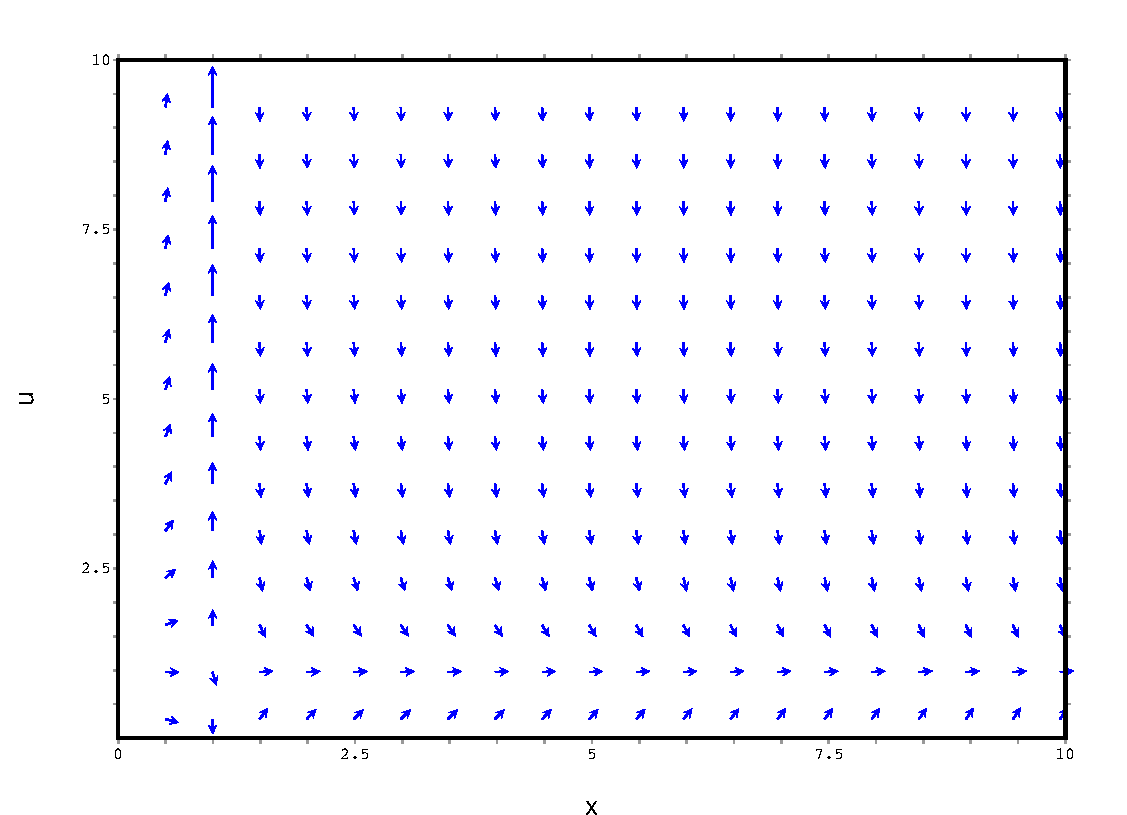
\includegraphics[width=7cm]{pictures/vector_field_1.pdf}
                    \caption{Векторное поле к уравнению (\ref{eq1})}
                \end{figure}
                
                \item 
                \( 
                    e^{xy} \cdot \left( y^2 + xyy' \right) = y' + y \cdot \cot{x}
                \)
                \label{eq2}

                \textit{Тип уравнения:}
                Уравнение, приводимое к уравнению в полных дифференциалах.

                \textit{Общее решение:}
                \( e^{xy} - \ln{y} - \ln(\sin{x}) = C. \)

                \textit{Векторное поле:}

                \begin{figure}[H]
                    \centering
                    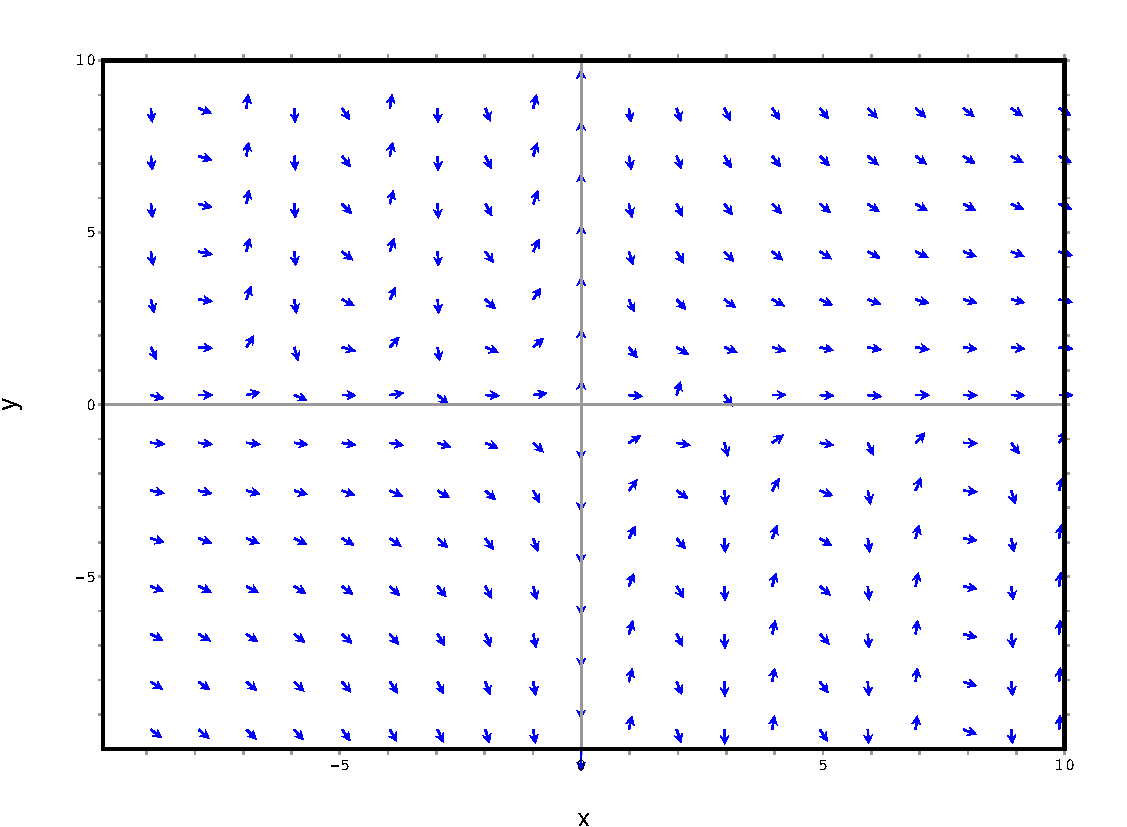
\includegraphics[width=7cm]{pictures/vector_field_2.pdf}
                    \caption{Векторное поле к уравнению (\ref{eq2})}
                \end{figure}
                
                \item 
                \( 
                    r' \cdot \cos^2{\varphi} = \sec{r} \cdot \ln{\sin{r}}.
                \)
                \label{eq3}

                \textit{Тип уравнения:}
                Уравнение с разделяющимися переменными.

                \textit{Общее решение:}
                \( \li{\sin{r}} = \tan{\varphi} + C. \)

                \textit{Векторное поле:}

                \begin{figure}[H]
                    \centering
                    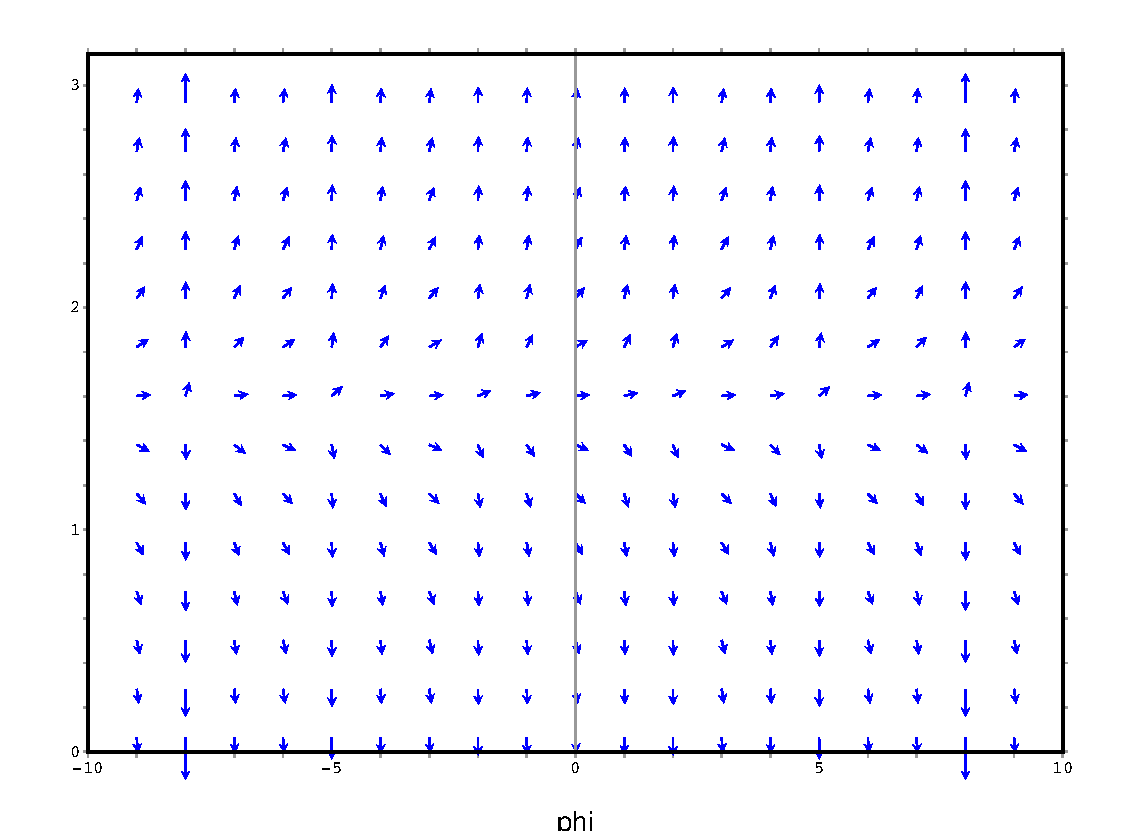
\includegraphics[width=7cm]{pictures/vector_field_3.pdf}
                    \caption{Векторное поле к уравнению (\ref{eq3})}
                \end{figure}
                
                \item 
                \( 
                    5x\sqrt{x} \cdot u' -5u\sqrt{x} = 25x^2 - u^2.
                \)
                \label{eq4}

                \textit{Тип уравнения:}
                Уравнение, приводимое к уравнению c разделяющимися переменными.

                \textit{Общее решение:}
                \(
                    \displaystyle
                    % \ln{ \left\vert \frac{u+5x}{u-5x} \right\vert } = 4 \sqrt{x} + C
                    \frac{u+5x}{u-5x} = C e^{4 \sqrt{x}}.
                \)

                \textit{Векторное поле:}

                \begin{figure}[H]
                    \centering
                    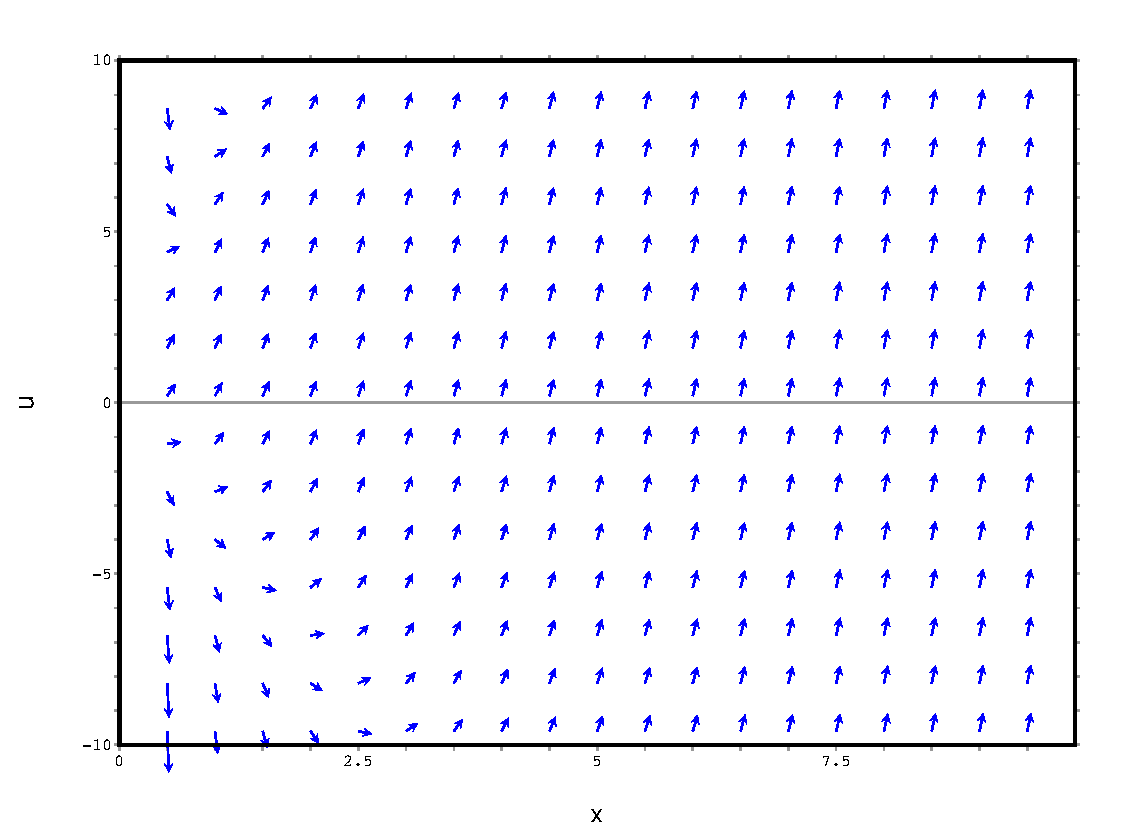
\includegraphics[width=6.5cm]{pictures/vector_field_4.pdf}
                    \caption{Векторное поле к уравнению (\ref{eq4})}
                \end{figure}
                
                \item 
                \(
                    y' \sqrt{x} \cdot \sec^2{\sqrt{y}} = 2\sqrt{y} \cdot 
                    \left( \tan{\sqrt{y}+\ln{x}} \right).
                \)
                \label{eq5}

                \textit{Тип уравнения:}
                Уравнение, приводимое к уравнению в полных дифференциалах.

                \textit{Общее решение:}
                \(
                    \displaystyle
                    e^{-2\sqrt{x}}\left( \tan(\sqrt{y}) + \ln{x} \right) = 2\Ei(-2 \sqrt{x}) + C.
                \)

                \textit{Векторное поле:}

                \begin{figure}[H]
                    \centering
                    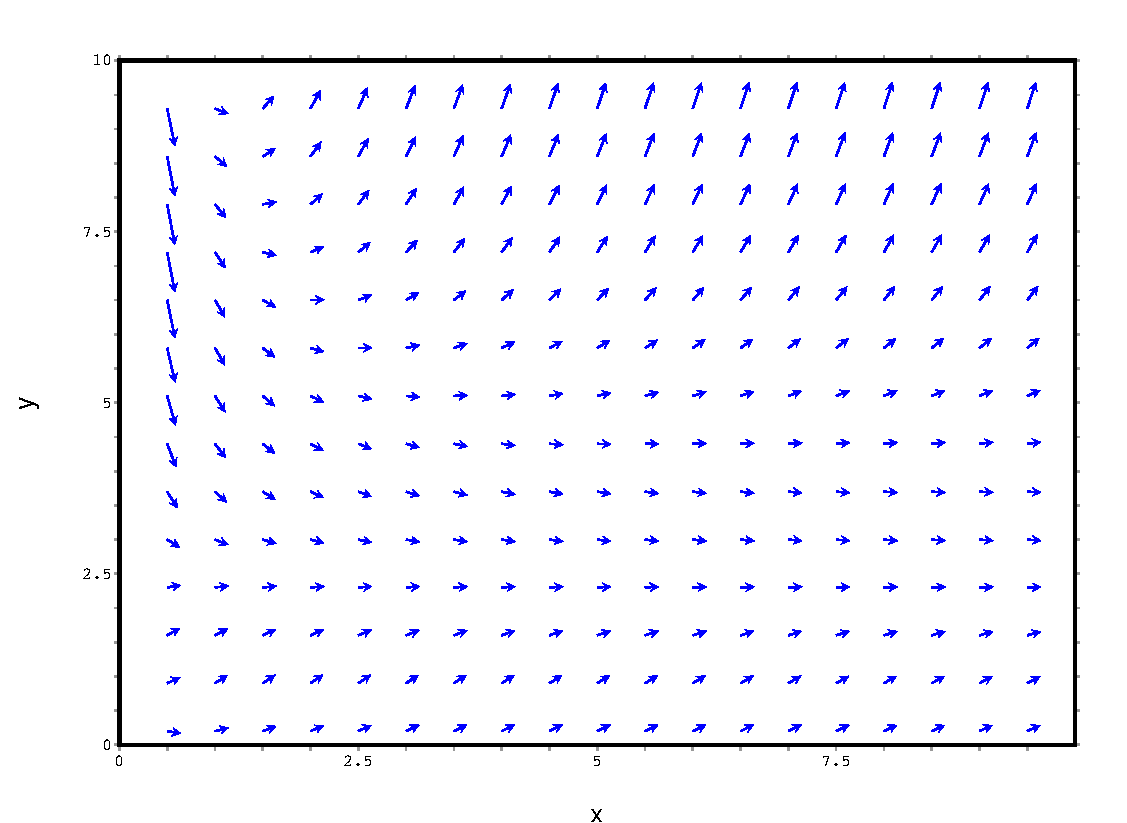
\includegraphics[width=6.5cm]{pictures/vector_field_5.pdf}
                    \caption{Векторное поле к уравнению (\ref{eq5})}
                \end{figure}
            \end{enumerate}

    
    \pagebreak

    \section{Задание 2: Решить задачи Коши}

        \subsection{Постановка задачи}
            Для следующих уравнений с начальными условиями определить тип, найти
            общее и частное решения, построить график решения и векторное поле уравнения:
        
            \begin{enumerate}
                \item
                \(
                    \displaystyle
                    \theta r' = \theta \cdot \sin{\frac{r}{\theta}} + r, ~ r(1) = \frac{\pi}{2}
                \)

                \item 
                \(
                    \displaystyle
                    y' \cos{x} + y = \frac{y}{\ln{y}}, ~ y(0) = 1 
                \)
            \end{enumerate}

        \subsection{Решение}

            \begin{enumerate}
                \item
                \(
                    \left\lbrace
                    \begin{aligned}
                        &\theta r' = \theta \cdot \sin{\frac{r}{\theta}} + r \\
                        &r(1) = \frac{\pi}{2}
                    \end{aligned}
                    \right.
                \)
                \label{eq6}

                \textit{Тип уравнения:}
                Уравнение, приводимое к уравнению с разделяющимися переменными.

                \textit{Общее решение:}
                \(
                    \displaystyle
                    \tan{\frac{r}{2\theta}} = C \theta.
                \)

                \textit{Частное решение:}
                \(
                    \displaystyle
                    \tan{\frac{r}{2\theta}} = \theta.
                \)

                \textit{Векторное поле:}

                \begin{figure}[H]
                    \centering
                    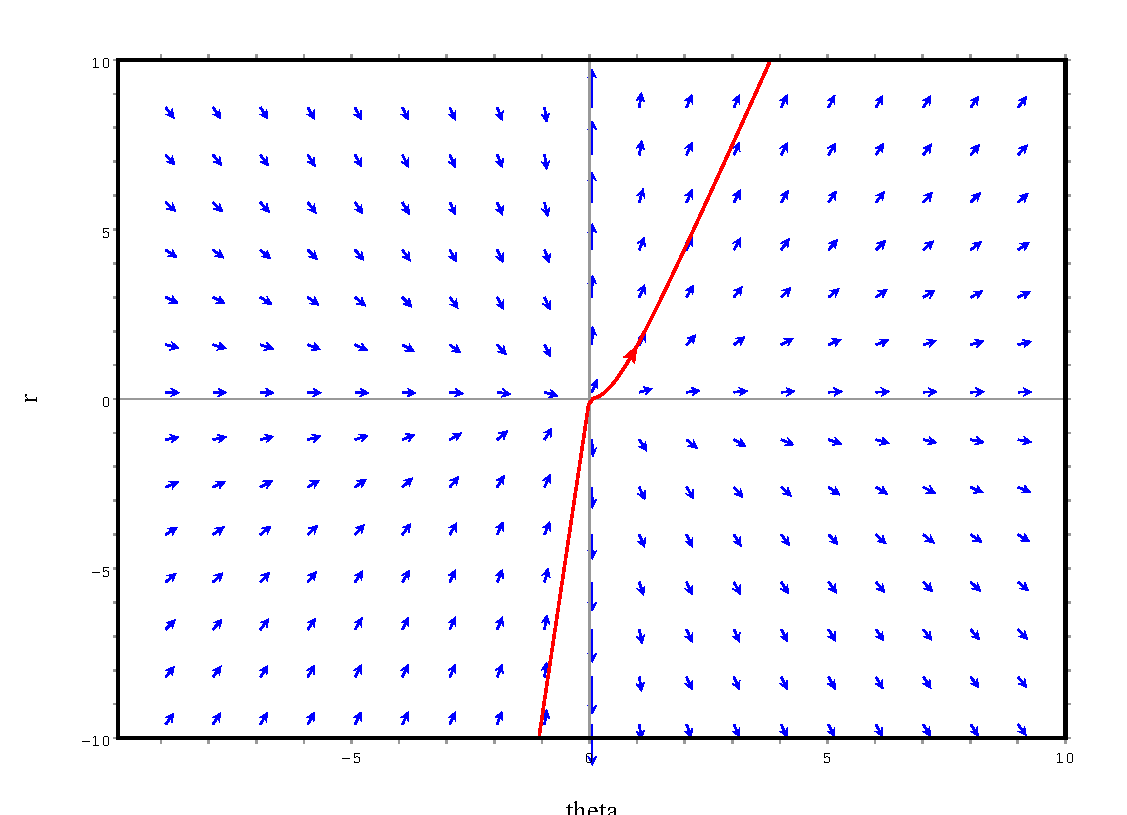
\includegraphics[width=6.5cm]{pictures/vector_field_6.pdf}
                    \caption{Векторное поле к уравнению (\ref{eq6})}
                \end{figure}

                \item 
                \(
                    \left\lbrace
                    \begin{aligned}
                        &y' \cos{x} + y = \frac{y}{\ln{y}} \\
                        &y(0) = 1 
                    \end{aligned}
                    \right.
                \)
                \label{eq7}

                \textit{Тип уравнения:}
                Уравнение с разделяющимися переменными.

                \textit{Общее решение:}
                \(
                    \displaystyle
                    y(1 - \ln{y}) \tan\left( \frac{x}{2} + \frac{\pi}{4} \right) = C.
                \)

                \textit{Частное решение:}
                \(
                    \displaystyle
                    y(1 - \ln{y}) \tan\left( \frac{x}{2} + \frac{\pi}{4} \right) = 1.
                \)

                \textit{Векторное поле:}

                \begin{figure}[H]
                    \centering
                    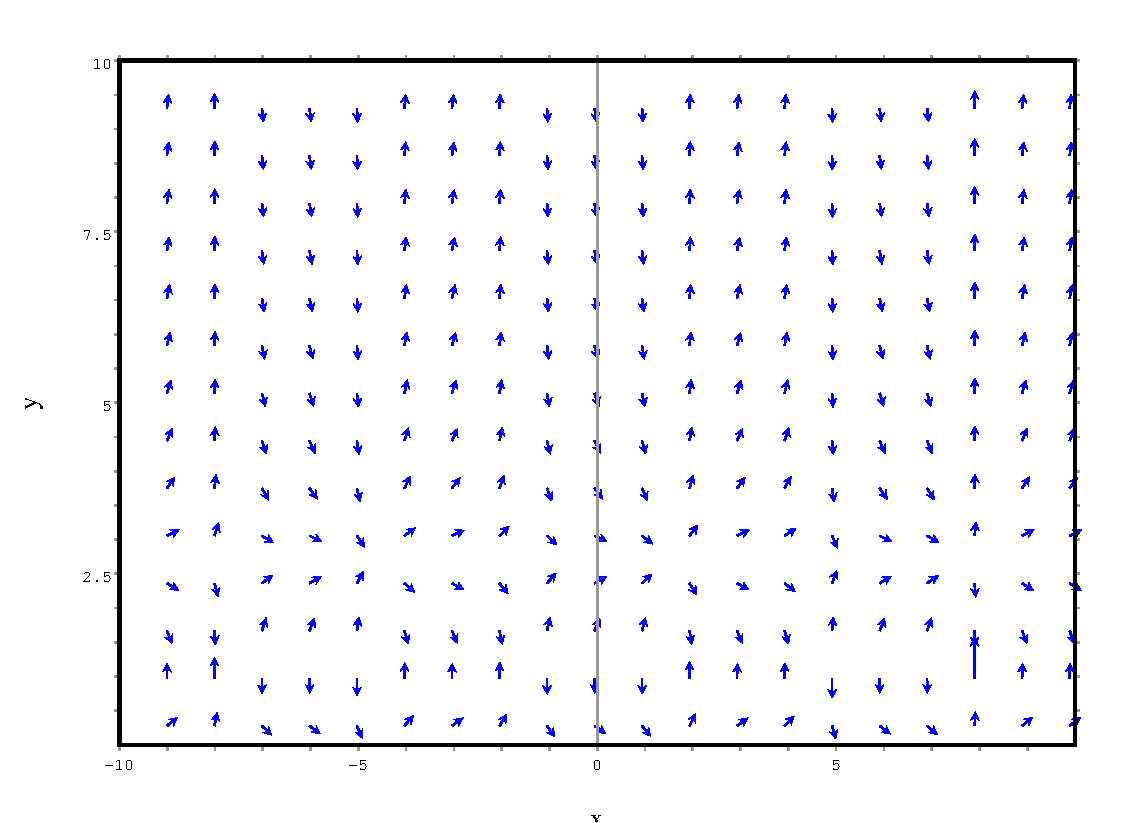
\includegraphics[width=6.5cm]{pictures/vector_field_7.pdf}
                    \caption{Векторное поле к уравнению (\ref{eq7})}
                \end{figure}
            \end{enumerate}

    \pagebreak

    \section{Задание 3: Проверка решения задачи Коши}

        \subsection{Постановка задачи}
            Для следующей задачи Коши проверить, является ее ли
            решением представленная неявно заданная функция:
            \[
                \theta r' \cdot \left( \theta - \sin{e^r} + r e^r \cdot \cos{e^r} \right)
                = \theta r - r^2, ~ r(1) = \ln{\frac{\pi}{2}}; \quad r \ln{\theta} + \sin{e^r} = \theta.
            \]

        \subsection{Решение}
            
        \textit{Проверка начальных условий:}

            \[ \ln{\frac{\pi}{2}} \ln{1} + \sin{e^{\ln{\frac{\pi}{2}}}} = 1 \]
            \[ 0 + 1 = 1 \]
            \[ 1 = 1 \]

        Решение удовлетворяет начальным условиям.

        \textit{Проверка решения уравнения:}

            \[ r' \ln{\theta} + \frac{r}{\theta} +  e^r r'\cos{e^r} = 1 \]

        Подставим
        \( 
            \displaystyle  
            \ln{\theta} = \frac{\theta - \sin{e^r}}{r}.
        \)
        
        \[ 
            r' \frac{\theta - \sin{e^r}}{r} +  e^r r'\cos{e^r} + \frac{r}{\theta} = 1 
            \quad \vert \cdot r \theta
        \]
        \[ \theta r' \left( \theta - \sin{e^r} + e^r r \cos{e^r} \right) + r^2 = r \theta \]
        \[ \theta r' \cdot \left( \theta - \sin{e^r} + r e^r \cdot \cos{e^r} \right) = \theta r - r^2 \]
    
        Дифференцируя решение, и используя зависимости между функциями в решении,
        было получено исходное уравнение.

        \textit{Ответ:} Неявно заданная функция является решением задачи Коши.
    \pagebreak

    \section{Заключение}
        В этой лабораторной работе мы решили дифференциальные
        уравнения, построили векторные поля, а также решили и проверили задачи Коши,
        сверстав решения в \LaTeX.


\end{document}